\documentclass{article}

% if you need to pass options to natbib, use, e.g.:
% \PassOptionsToPackage{numbers, compress}{natbib}
% before loading nips_2018

% ready for submission
\PassOptionsToPackage{numbers}{natbib}
\usepackage[final]{../common/nips_2018}

% to compile a preprint version, e.g., for submission to arXiv, add
% add the [preprint] option:
% \usepackage[preprint]{nips_2018}

% to compile a camera-ready version, add the [final] option, e.g.:
% \usepackage[final]{nips_2018}

% to avoid loading the natbib package, add option nonatbib:
% \usepackage[nonatbib]{nips_2018}

\usepackage[utf8]{inputenc} % allow utf-8 input
\usepackage[T1]{fontenc}    % use 8-bit T1 fonts
\usepackage{hyperref}       % hyperlinks
\usepackage{url}            % simple URL typesetting
\usepackage{booktabs}       % professional-quality tables
\usepackage{amsfonts}       % blackboard math symbols
\usepackage{nicefrac}       % compact symbols for 1/2, etc.
\usepackage{microtype}      % microtypography
\usepackage{graphicx}

\title{CS224n Project Proposal}

% The \author macro works with any number of authors. There are two
% commands used to separate the names and addresses of multiple
% authors: \And and \AND.
%
% Using \And between authors leaves it to LaTeX to determine where to
% break the lines. Using \AND forces a line break at that point. So,
% if LaTeX puts 3 of 4 authors names on the first line, and the last
% on the second line, try using \AND instead of \And before the third
% author name.

\author{
  Luis A. Perez \thanks{} \\
  Department of Computer Science\\
  Stanford Univeristy\\
  Stanford, CA 94305 \\
  \texttt{luis0@stanford.edu} \\
  %% examples of more authors
  %% \And
  %% Coauthor \\
  %% Affiliation \\
  %% Address \\
  %% \texttt{email} \\
  %% \AND
  %% Coauthor \\
  %% Affiliation \\
  %% Address \\
  %% \texttt{email} \\
  %% \And
  %% Coauthor \\
  %% Affiliation \\
  %% Address \\
  %% \texttt{email} \\
  %% \And
  %% Coauthor \\
  %% Affiliation \\
  %% Address \\
  %% \texttt{email} \\
}

\begin{document}
% \nipsfinalcopy is no longer used

\maketitle

\begin{abstract}
  In this paper, we explore several extensions of BERT for the Stanford Question and Answer v2.0 task in NLP, and summarize our analyzes of these results. In particular, we explore the benefits of using a fined-tuned BERT model for word-embdeddings underlying different, more complex question-and-answer architectures. We begin by setting a baseline system where BERT is used with a single additional layer, fine-tuned on the SQuAD dataset as presented in the original paper \cite{BERT}. We demonstrate that such a system achieves great performance, as measures by F1, EM, and Answer-vs-No-Answer (AvNA) metrics. We continue by exploring different more traditional QA architectures, such as a BiDAF and a few other customized models. Additionally, we experiment with replacing the BERT embeddings with GPT-2 \cite{GPT2}. Finally, we conclude by performing an analysis of our results and experiments, and provide guidence of the future direction of this work.
\end{abstract}

\section{Approach}
In the paper by Jacob Devlin, Ming-Wei Chang, Kenton Lee, and Kristina Toutanova from the Google AI Language Lab titled ``BERT: Pre-training of Deep Bidirectional Transformers for Language Understanding'' \cite{BERT}, BERT, an LM, is shown to have great promise in a wide variety of tasks. In particular, it perform extremenly well on the SQuAD v2.0 challenge. See Table \ref{table:top_10_squad} for a list of the top-ten models, and note that all of these models make use of the BERT architecture + weights as a foundation for their work. 

BERT is a pre-trained, non-task-specific language model which has been used to further the SOTA results in task-specific metrics, such as GLUE and SQuAD v1.1. Other similar language models exists, such as ELMO \cite{ELMO} and GPT-2 \cite{GPT2}, each making use of a large corpus of language traning data in order to generate \textit{deep contextualized} word representations, rather than static, fixed-size word representations used previously, such as those in word2vec. These representations can better model complex characteristics of word use and how these uses vary across lingustic contexts. BERT, specifically, follows the same core idea as ELMO -- extending the embeddings for a word be using the context in which it appears to modify them. All of these large language models vary mostly in the architecture of the neural networks.  

With these pre-trained language representations, task-specific models can be utilized downstream through two main strategies (1) feature-based and (2) fine-tuning. The former essentially includes the pre-trained language representations along with additional features, to train a new model, while the latter simply fine-tunes the pre-trained parameters (without introducing too many new parameters).


\subsection{Detailed Architecture}
The BERT paper \cite{BERT} specifically tries to solve the problem of learning an improved language model for use in word-representations. In this paper, we take a similar approach and extend it. We use the pre-trained version of the BERT weights, which have been ported to PyTorch \footnote{\href{https://github.com/huggingface/pytorch-pretrained-BERT}{PyTorch Open-Source Port of Multiple Models}}. We provide a brief overview of the architecture and the pre-training tasks.

The BERT embeddings are context-aware and are contructed from two tasks.
\begin{itemize}
    \item The ``masked language model''. 
    \item The ``next sentence prediction''.
\end{itemize}

With these pre-training objectives independent of final objectives, (2) utilization of bi-directional models to take full advantage of the language model, and (3) a pre-trained model which achieves SOTA results across multiple, distinct NLP tasks after fine-tuning, with a single additional layer. The key achievement is a 4.4\% to 6.7\% average accuracy improvement over previous SOTA models in the GLUE benchmarks. The full results (for all benchmarks) are reproduced in Table \ref{fig:bert_glue_results} from the paper. The best performing BERT system also outperforms the top leaderboard system by +1.5 F1 in ensembling and +1.3 F1 on a single system. For more details, see Table \ref{fig:bert_squad_results}. In this paper, we use these original values as our baselines.

BERT's model architecture is simply a multi-layer bidrectional Transformer encoder based on the original implementation by Vaswani et al \cite{AttentionIsAllYouNeed} and as detailed in Figure \ref{fig:bert_architecture_comparison}. Transformers help reduce the number of operations required to learn long-distance dependencies to a constant number (at the cost of resolution). They make use of stacked self-attention and point-wise, FC layers for the encoder and decoder, as can be seen in Figure \ref{fig:transformers}. A detailed discussion of this architecture (by annotating the paper that introduced it), can be found \href{http://nlp.seas.harvard.edu/2018/04/03/attention.html}{here}.

This model is then trained on the BooksCorpus (800M words) and English Wikipedia (2,500M words) (only text, no lists/tables/headers). The model we use is trained on the MLM task. In this context, the input data has tokens randomly masked (removed), and the goal is to generate a model that, given this incomplete data, can correctly identify the original vocabulary id. One key aspect of this task is that the model has access to both previous words \textbf{and} future words. Further, it is different from auto-regressive models in that only the hidden state for the masked-word is used to compute the softmax probabilities over the vocabulary. We defer further details in this task to \cite{BERT}, but suffice it to say that the learned, context-aware embeddings are quite effective at capturing the most important properties of language.

\subsubsection{Our Modifications}
All of our code for the experiments is publically available \href{https://github.com/kandluis/cs224n}{here}. The paper explores two main objectives, all of which rely on pre-trained contextualized embeddings:

\begin{enumerate}
  \item Network architecture comparison for fine-tuning [single-layer model, BiDAF, QANet] of BERT word-embeddings.
  \item Contextualized word-embedding effect [ELMo vs BERT vs GPT-1 vs GPT-2] on most promising architecture.
  \item Hyperparameter tuning during training using Bayesian Learning (see \href{https://github.com/HIPS/Spearmint}{Spearmint Package}) on BERT + BiDAF
\end{enumerate}

\subsubsection{Network Architecture Comparisons}
With the network architecture comparison, we see to understand the effect of further network architectures on-top of pre-trained contextual word-embeddings. In particular, this paper answer the following questions.

\begin{itemize}
    \item Do we need fine-tuning layer? Here, we propose an extreme, where we actually seek to analyze and understand the results of using BERT with no additional fine-tuning layers.
    \item What if it were deeper? Here, we propose an extension, where additional intermediate convolutional layers are used rather than a single FC layer on the classification hidden state. We suspect that this will lead to some improved performance on the fine-tuned tasks, since the model will have increased flexibility and capacity.
    \item Can we make use of the other transformer hidden states? Our hypothesis is that currently fine-tuned BERT models are bottlenecked by the single hidden-state. Instead, we propose making use of all of the transformer hidden states for classification
\end{itemize} 

The key contribution in our paper is mostly experimental. We begin by using the BERT word-embeddings with full-network fine-tunining to perform question-and-answering. Our baseline model consists of exactly this model. We have already trained this model \footnote{\href{https://github.com/kandluis/cs224n}{code}}.

\subsubsection{Linear Model}
For this system, we take advantage of the input representation used by BERT. The question tokens correspond to the sentence 1 encoding, and the paragraph to the sentence 2 encoding. Then each output transform state, $T_i$ is dot-produced with two new parameter vectors, $S$ and $E$ for start and end. The a straightforward softmax is taken from this dot-product for all $i$, to determine the start and end of the corresponding answer in the text. Similar modifications are used for other tasks, which are detailed further in the paper. 

The metric would be to use BLEU against the correctly extracted sentence text. In a failure mode, the model would actually learn simply to find the answer text and generate it. However, we'd like to avoid this happening. 

\subsubsection{BiDAF Model}
For this system, we compare the performance of BERT embeddings using a more complex model on top. In particular, we make use of the BiDAF model which makes use of highway layers as well as other layers in order to improve in the context of question and answering.

\subsubsection{Custom Model}
For the final comparison, we make use of a model which consists of a simple additional attention mechanism on the embeddings produced by BERT.


\section{Experiments}
Current experimental results have been submitted to the PCE-division of the DEV board and consists only of having full-trained a baseline model using the BERT context embeddings. Training was done for 2 epochs, and achieved decent results (though not as claimed in the original paper). This is likely due to fine-tuning for only 2 epochs.

\subsection{Concrete Results and Other Parameters}
For the training of the base-line model we used the same parameters as specified in the original paper \cite{BERT}. In particular, we trainined our models for a total of 2 epochs (for fine-tuning).

\begin{enumerate}
  \item Only fine-tuning the final layers. This took on the order of ~2 hours on 2 GPUs. This achieved EM: 50.921 (+50.921) and F1: 50.996 (+50.996), which is actually worse than the provided baselines. We used learning reate of 1e-5 with a fixed schedule. 
  \item Fine-tuning the entire BERT model in addition to the final layer. This took on the order of ~10 hours on 2 GPUs and achieved our best results so far, with a score of EM: 72.688 (+21.767) and F1: 76.071 (+25.075). 
\end{enumerate}

We performed additional experiments, but none which have demonstrated any promising approaches. We're currently still running experiments on the BiDAF model with BERT embeddings.t

\subsection{Result Evaluation}
As discussed above, SQuAD v2.0 will be used as the default, automatic evaluation metric for all of the modifications proposed above (for the SQuAD task). 

\section{Future Work}
This section is still to be completed. In particular, we're interested in training the same models above but using different embeddings. Specifically, it will be useful to make use of the GPT-2 pre-trained models recently released by OpenAI. Furthermore, we'd like to make use of Bayesian Hyper Parameter optimization \textit{during} training -- in particular, in regards to the learning rate schedule. Specifically, we'd like to have the learning rate schedule dynamic, but not-prespecified, but rather learned based on each batch of data.

\subsection{Concluding Remarks}
Overall, the paper presents an attention-based mechanism for pre-training on a large-corpus of data. Furthermore, due to the architectural choices and the input representations, this pre-trained model called BERT can be fine-tuned, with the addition of a few final layers, to achieve SOTA performance across many tasks. 


\section{Appendix}

\begin{table}[!ht]
\centering
\begin{tabular}{l|l|l|l}
Model/Method                   & Category       & EM     & F1     \\ \hline
BERT + MMFT+ ADA               & BERT Ensemble  & 85.082 & 87.615 \\
BERT + Synthetic Self-Training & BERT Ensemble  & 84.292 & 86.967 \\
BERT finetune baseline         & BERT Ensemble  & 83.536 & 86.096 \\
Lunet + Verifier + BERT        & BERT Ensemble  & 83.469 & 86.043 \\
PAML + BERT                    & BERT Ensemble  & 83.467 & 86.035 \\
Lunet + Verifier + BERT        & BERT Extension & 82.995 & 86.035 \\
BERT + MMFT + ADA              & BERT Extension & 83.040 & 85.892 \\
BERT + Synthetic Self-Training & BERT Extension & 82.975 & 85.810 \\
PAML + BERT                    & BERT Extension & 82.577 & 85.810
\end{tabular}
\caption{Table with Top 10 models/methods on SQuAD 2.0 as of 2/12/2019. See \href{https://rajpurkar.github.io/SQuAD-explorer/}{SQuAD Leaderboard} for more details.}
\label{table:top_10_squad}
\end{table}

\begin{figure}[!ht]
\centering
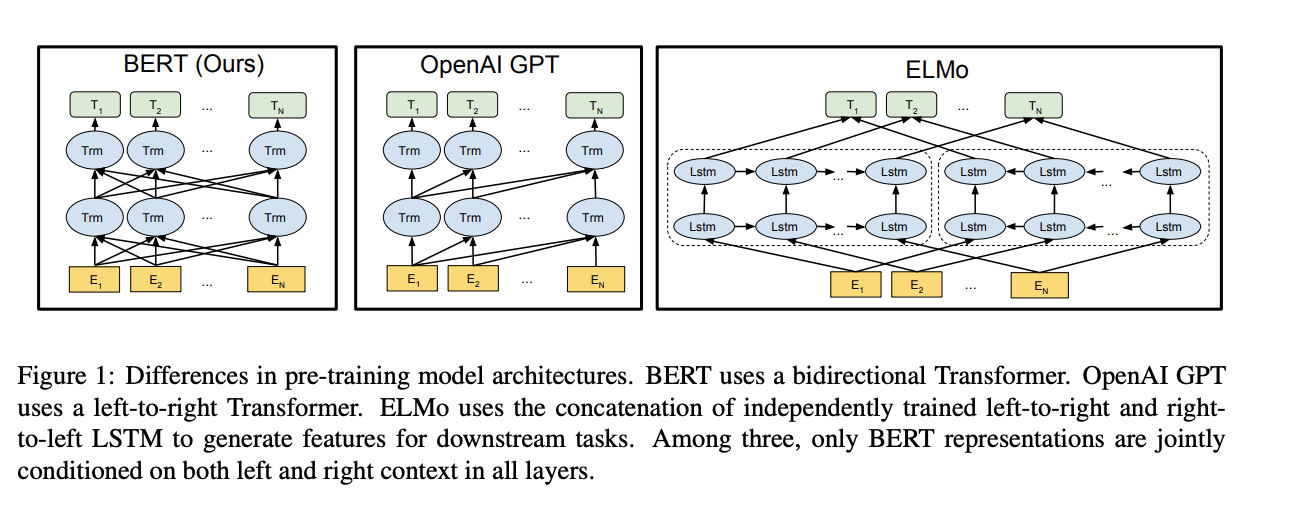
\includegraphics[scale=0.7]{../figures/BERT_architecture_comparsion}
\label{fig:bert_architecture_comparison}
\end{figure}


\begin{figure}[!ht]
\centering
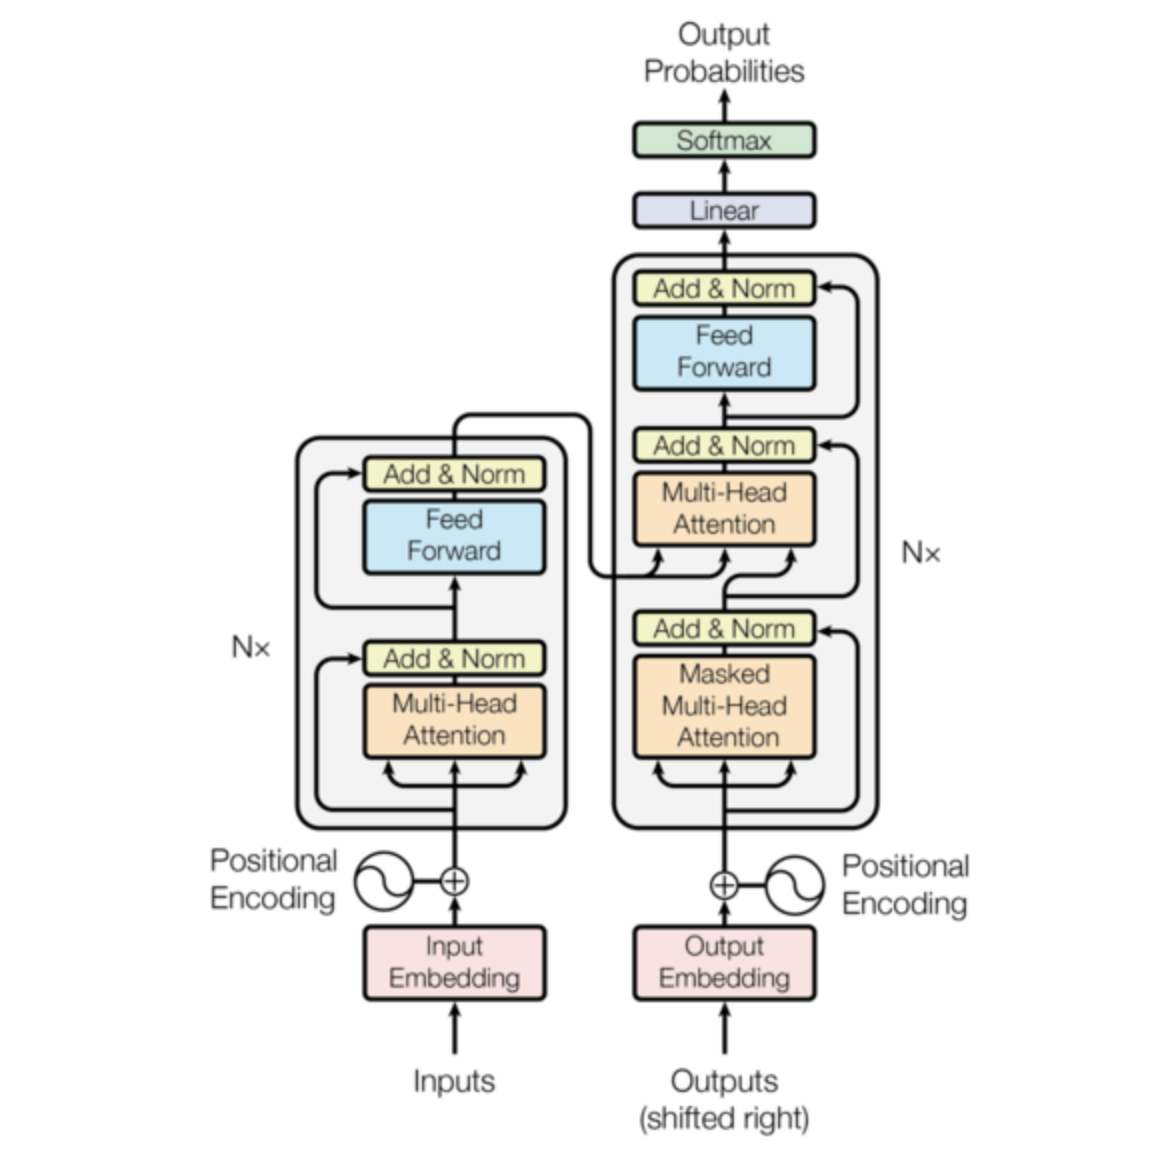
\includegraphics[scale=0.7]{../figures/Transformers}
\label{fig:transformers}
\end{figure}

\begin{figure}[!ht]
\centering
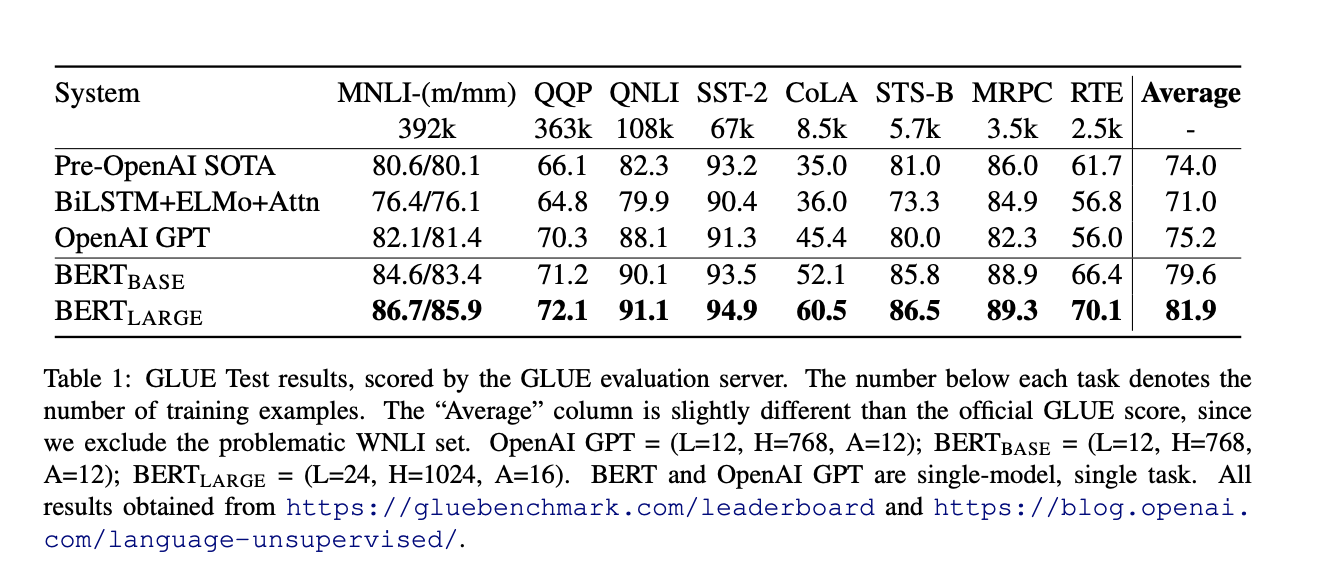
\includegraphics[scale=0.7]{../figures/BERT_GLUE_results}
\label{fig:bert_glue_results}
\end{figure}

\begin{figure}[!ht]
\centering
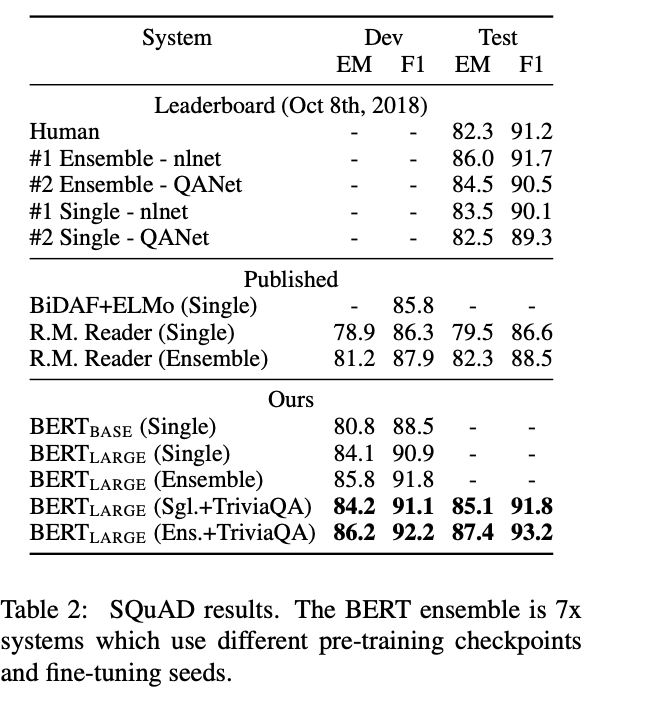
\includegraphics[scale=0.7]{../figures/BERT_SQuAD_results}
\label{fig:bert_squad_results}
\end{figure}

\section*{References}

{\small
\bibliographystyle{../common/ieee}
\bibliography{../common/egbib}
}

\end{document}
